% Created 2022-05-05 Thu 07:02
% Intended LaTeX compiler: pdflatex
\documentclass[bigger]{beamer}
\usepackage[utf8]{inputenc}
\usepackage[T1]{fontenc}
\usepackage{graphicx}
\usepackage{longtable}
\usepackage{wrapfig}
\usepackage{rotating}
\usepackage[normalem]{ulem}
\usepackage{amsmath}
\usepackage{amssymb}
\usepackage{capt-of}
\usepackage{hyperref}
\usetheme{default}
\author{Diamond Bond}
\date{\today}
\title{Bugzilla}
\hypersetup{
 pdfauthor={Diamond Bond},
 pdftitle={Bugzilla},
 pdfkeywords={},
 pdfsubject={},
 pdfcreator={Emacs 29.0.50 (Org mode 9.5.3)}, 
 pdflang={English}}
\begin{document}

\maketitle
\begin{frame}{Outline}
\tableofcontents
\end{frame}


\section{What is it?}
\label{sec:orge29e877}
\begin{frame}[label={sec:orgc23cd51}]{Description}
A minimalistic Bug report tracker written in C++ for Windows \& Linux.

\begin{center}
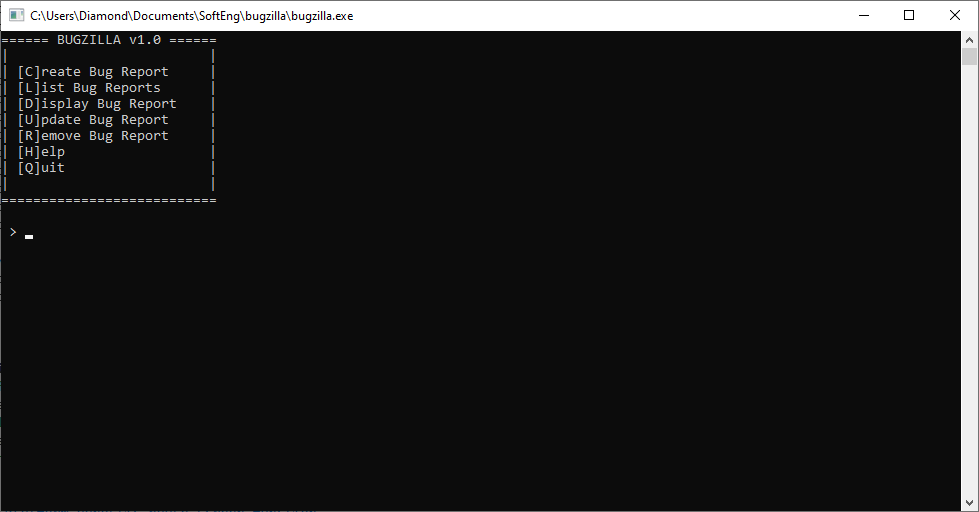
\includegraphics[width=.9\linewidth]{../img/mainmenu.png}
\end{center}
\end{frame}

\section{Features}
\label{sec:org657c50b}

\begin{frame}[label={sec:org1cf137d}]{Create a bug report}
This function prompts the user for a filename then proceeds to create the file.
It then asks the user for the relevant information pertaining to a bug report.
\end{frame}

\begin{frame}[label={sec:org151c09c}]{List bug reports}
This function lists the available bug reports, we expose it to the user so they can utilize it as they best see fit.
We also utilize this function internally before filename selection in other functions, this helps provide the user with some context as to what files are available to be read from.
\end{frame}

\begin{frame}[label={sec:orge3dc7f0}]{Display a bug report}
This function displays a bug report in a formatted way.
It also calls upon list reports before asking for a filename to ensure the user knows that filenames (bug reports) exist.

note: The file name list is taken from the CWD (current working directory)
\end{frame}

\begin{frame}[label={sec:org17391ac}]{Update a bug report}
This function lists out possible bug reports, asks the user to select one (via inputting the filename).
It then proceeds to print out the old information then asks the user for the newly updated bug report information.

note: Careful consideration has gone into what fields / info can \&/or should be updated so as to avoid mangling the important information that was created (eg: Created At time and original filename)
\end{frame}

\begin{frame}[label={sec:orgd2e98e8}]{Remove a bug report}
Prompts the user for filename after listing possible filenames.
Deletes the filename that was provided by the user if it exists and prints out a success message otherwise it prints an error message.
\end{frame}

\begin{frame}[label={sec:org6638927}]{Help}
\begin{center}
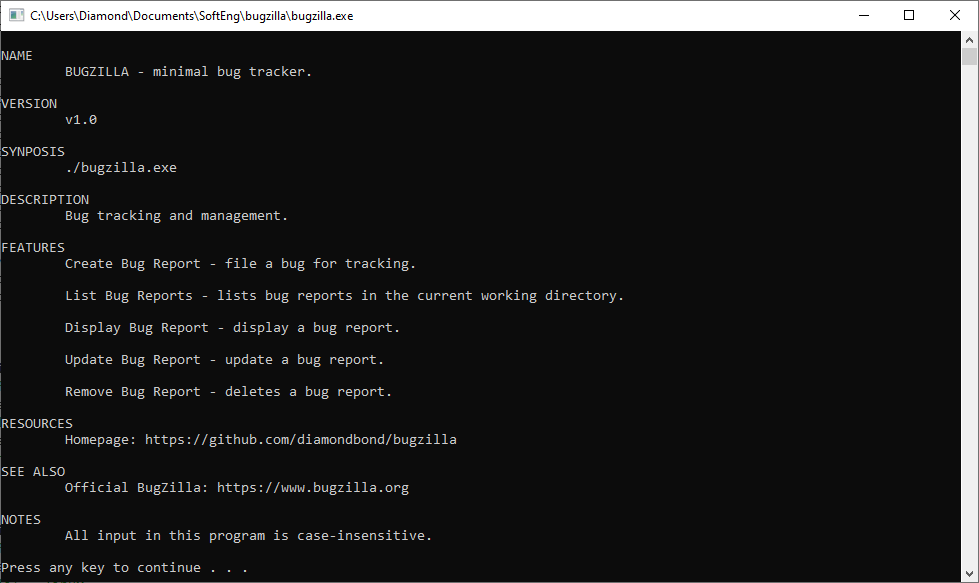
\includegraphics[width=.9\linewidth]{../img/help.png}
\end{center}
\end{frame}

\section{Inspiration}
\label{sec:org60af09c}
\begin{frame}[label={sec:orge0fc65d}]{A Brief History of Bugzilla}
This project was insipired by the original \href{https://www.bugzilla.org}{Bugzilla}.

When mozilla.org first came online in 1998, one of the first products that was released was Bugzilla, a bug system implemented using freely available open source tools. Bugzilla was originally written in TCL by Terry Weissman for use at mozilla.org to replace the in-house system then in use at Netscape. 
\end{frame}

\begin{frame}[label={sec:org6204bc4}]{Links}
Homepage: \url{https://github.com/diamondbond/bugzilla}

Original Bugzilla: \url{https://www.bugzilla.org/about}
\end{frame}
\end{document}